% =============================================================================
% Item D do roteiro (Aula 14): estudo de aproveitamento técnico.
% Base empírica: quadro da Galeria no Miro, https://miro.com/app/board/uXjVEe1I-Mw=/
% (lido em 04/10/2026): 18 painéis, 101 efeitos físicos, 126 portadores,
% 27 rótulos "explorar" e 22 notas da equipe.
% Figura: imagens/aproveitamento_tecnico/galeria_painel_F1-1.pdf
% A combinação dos princípios em alternativas e a arquitetura (item E do
% roteiro) ficam na Seção 14 (sec:reformulacao_desenhos).
% =============================================================================

\section{ESTUDO DE APROVEITAMENTO TÉCNICO}\label{sec:aproveitamento_tecnico}

O estudo de aproveitamento técnico levantou as ideias que a equipe pode aproveitar de produtos já existentes. Ele partiu de duas bases: as funções da modelagem funcional (Seção~\ref{sec:modelagem_funcional}), que descrevem o sistema sem referência a princípios físicos, e o benchmarking das soluções concorrentes, feito no estudo de diferenciação (Seção~\ref{sec:estudo_diferenciacao}).

Para cada função, a equipe procurou meios físicos capazes de cumpri-la. \citeonline{rozenfeld2006gestao} chamam essa atividade de desenvolver princípios de solução para as funções e a situam na passagem da função à forma. A busca respondeu a três perguntas: que efeitos físicos cumprem a função, que sistema concreto porta cada efeito e em que produto esse sistema já funciona.

O levantamento reuniu 101 efeitos físicos e 126 portadores nas 18 funções da estrutura (Figura~\ref{fig:estrutura_funcoes}). As referências vieram de seis linhas de similaridade, e 27 ideias foram selecionadas para a etapa seguinte. A combinação dessas ideias em alternativas de concepção, por meio da matriz morfológica, fica na reformulação dos desenhos (Seção~\ref{sec:reformulacao_desenhos}).

\subsection{Planejamento do levantamento de princípios de solução}
\label{subsec:aprov_fundamentacao}

Segundo \citeonline{rozenfeld2006gestao}, um princípio de solução combina um efeito físico, que explica por que a função pode ser cumprida, e um portador do efeito, sistema físico definido de forma qualitativa por seus elementos e pelas relações entre eles. Uma função admite vários efeitos, e cada efeito admite vários portadores. O portador indica tipo, quantidade, forma, posição e movimento dos elementos, sem fixar o material específico nem as dimensões.

A disciplina apresentou três fontes de princípios de solução: bancos de dados, catálogos e métodos de criatividade, como o \textit{brainstorming}, a galeria e o método morfológico. Na galeria, que os autores classificam como método intuitivo, cada integrante propõe soluções individualmente, por meio de desenhos e textos fixados numa parede, e o grupo analisa as propostas em seguida. A equipe adotou a galeria para gerar os princípios de solução de cada função.

Cada proposta recebeu a forma dessa decomposição: todo cartão nomeia um efeito físico ou um portador ligado a um efeito. Com isso, as ideias de uma mesma função ficam no mesmo nível de generalidade, condição que o procedimento da matriz morfológica recomenda para a lista de princípios de cada função \cite[Quadro 7.4]{rozenfeld2006gestao}. Como a equipe montou uma parede por função, cada parede corresponde a uma linha candidata da futura matriz.

A cada portador, a equipe associou uma referência: um produto em que aquele sistema já funciona, na mesma função ou numa função análoga. As referências são o benchmarking deste estudo e foram agrupadas em linhas de similaridade (Seção~\ref{subsec:aprov_linhas}). Na geração de ideias, o grupo também consultou uma ferramenta de inteligência artificial para explorar princípios de solução alternativos e discutir soluções potenciais, por meio do plugin \texttt{/brainstorm} da Anthropic para \textit{Product Management}.

\subsection{Galeria de ideias}
\label{subsec:aprov_galeria}

A galeria ocupou um quadro do Miro intitulado ``PRO3474 · Galeria de ideias · efeitos e portadores''. O quadro tem uma parede, aqui chamada de painel, para cada uma das 18 funções secundárias necessárias e acessórias da estrutura de funções. Os painéis seguem a estrutura: uma fileira para os desdobramentos de \emph{reter a peça} (F1.1 a F1.3), outra para os de \emph{vincular a peça ao pagamento} (F2.1 a F2.5), outra para os de \emph{liberar a peça} (F3.1 a F3.4), uma para as funções acessórias (A1 a A5) e um painel para a função auxiliar F0. As funções básicas F1, F2 e F3 entram por meio de seus desdobramentos. O quadro materializa a parede da galeria: as propostas, em texto e com um pictograma, ficam fixadas por função, e a análise do grupo aparece nos rótulos de avaliação, nas revisões e nas notas assinadas.

Cada painel abre com os fluxos de entrada e saída da função, coerentes com a estrutura de funções (em F1.1, ``Entra: peça livre. Sai: peça retida''), e as propostas respondem a essa transformação. À esquerda fica a função; à direita, os cartões cinzentos de efeito físico, cada um com o nome do efeito e uma frase que explica o fenômeno, acompanhado de um pictograma; abaixo de cada efeito, os cartões de portador. O cartão de portador tem campos fixos: \emph{Como}, que descreve os elementos do sistema e as relações entre eles; \emph{Ref.}, a referência de produto; \emph{Revisão}, o julgamento do grupo; e, quando o uso tem restrição, \emph{Condição}. A Figura~\ref{fig:aprov_painel} reproduz parte do painel F1.1.

\begin{figure}[htbp]
    \centering
    \caption{Recorte do painel F1.1 (\emph{iniciar a retenção da peça}) do quadro da Galeria, com dois efeitos físicos, quatro portadores avaliados e duas notas da equipe}
    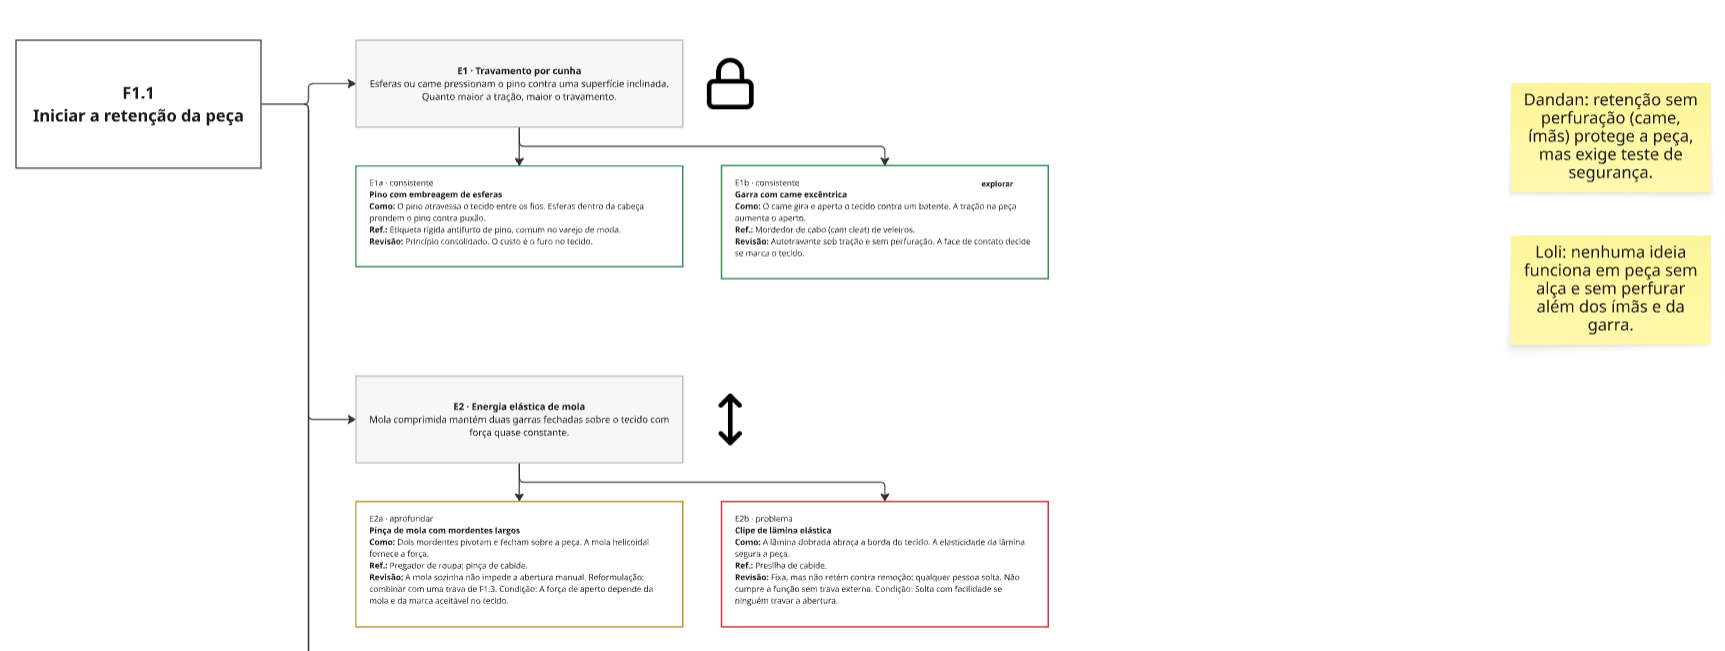
\includegraphics[width=\textwidth]{imagens/aproveitamento_tecnico/painel_galeria.png}
    \label{fig:aprov_painel}
    \source{Elaborado pelos autores (2026), a partir do quadro da Galeria no Miro. Textos, cores e ligações reproduzidos do quadro; as notas foram aproximadas dos cartões.}
\end{figure}

No recorte, o efeito E1, travamento por cunha, recebeu dois portadores consistentes: o pino com embreagem de esferas, tirado das etiquetas rígidas antifurto, e a garra com came excêntrica, tirada do mordedor de cabo de veleiros. A garra retém sem perfurar o tecido, vantagem destacada numa das notas, e recebeu o rótulo explorar. Em E2, a pinça de mola ficou a aprofundar, com a proposta de combiná-la a uma trava de F1.3, e o clipe de lâmina terminou como problema, porque qualquer pessoa o solta. Em E3, fora do recorte, os dois arranjos de ímãs dependem de ensaio: o par de ímãs perde a segurança diante de um ímã externo mais forte.

A análise em grupo, segundo momento da galeria, usou a legenda do próprio quadro. Com três rótulos, o grupo julgou cada portador frente à função: \emph{consistente}, quando cumpre a função e tem referência conhecida; \emph{aprofundar}, quando é plausível, mas falta dado, teste ou confirmação; e \emph{problema}, quando apresenta falha técnica ou conceitual. Um quarto rótulo, \emph{explorar}, marcou as ideias que seguem para os princípios de solução e pode acompanhar um cartão consistente ou um cartão a aprofundar. Os cartões com problema permanecem no quadro, como a legenda determina, e o campo \emph{Revisão} guarda o motivo de cada descarte.

O grupo registrou notas com pareceres individuais sobre o quadro-geral de uma função. Algumas comparam portadores (``giroscópio e magnetômetro pouco acrescentam ao acelerômetro'', em A1); outras ligaram o quadro a dores relatadas pela loja, como a estação de pareamento que ``acrescenta tempo ao recebimento'' (F1.2), ou à acessibilidade (``cor não funciona para daltônicos'', em A3).

Durante a análise, a equipe reformulou três portadores: a pinça de mola de F1.1 passou a depender de uma trava de F1.3; o atuador piezoelétrico de F3.2, de curso curto demais para soltar um trinco, virou candidato a gatilho da mola pré-tensionada; e o corpo de polímero rígido de F1.3 passou a valer como especificação-meta, porque a resistência do material se aplica a qualquer portador e, como anotou o grupo: ``vai para as especificações''. Revisões e notas apontam ainda dependências entre funções que a combinação na matriz morfológica terá de respeitar. O pino de dentes flexíveis de F1.1 só funciona com um par definido em F3.2; a liberação por fluido magnetorreológico de F3.2 depende da mesma validação da trava de F1.3; e os registros irreversíveis de F2.4, a marcação a laser e o papel térmico, não têm par em F2.5, que precisa desfazer o vínculo no estorno. Por fim, a equipe conferiu as propostas contra a decisão, registrada na modelagem funcional, de indicar a liberação por luz: nas revisões da tinta eletrônica e do filme eletrocrômico de F3.3, o grupo registrou o conflito, porque esses portadores não emitem luz.

A mesma legenda valeu para os cartões que trazem a marca de um revisor. Quase todos ocupam o fim dos painéis, e a maioria traz efeitos pouco usuais no varejo, como vácuo, eletroadesão, fluido magnetorreológico, comunicação pelo corpo e quimioluminescência. Nove deles terminaram como problema, e sete receberam o rótulo explorar.

A Tabela~\ref{tab:aprov_galeria} resume o resultado da análise por painel. O painel de informar o estado da peça ao antifurto existente (F3.4) foi o único sem nenhum portador consistente, porque quase todos dependem da tecnologia do portal de saída, que a equipe ainda não confirmou com a Riachuelo.

\begin{table}[H]
    \centering
    \caption{Efeitos físicos e portadores por painel da Galeria, com a avaliação dos portadores}
    \label{tab:aprov_galeria}
    \footnotesize
    \renewcommand{\arraystretch}{1.2}
    \begin{tabularx}{\textwidth}{@{}
        >{\RaggedRight\arraybackslash}p{1.0cm}
        >{\RaggedRight\arraybackslash}X
        c c c c c c@{}}
        \toprule
        \textbf{Painel} & \textbf{Função} & \textbf{Efeitos} & \textbf{Portadores} & \textbf{Consist.} & \textbf{Aprof.} & \textbf{Probl.} & \textbf{Explorar} \\
        \midrule
        F1.1 & Iniciar a retenção da peça & 7 & 11 & 3 & 5 & 3 & 2 \\
        F1.2 & Associar a retenção à identidade da peça & 4 & 8 & 4 & 3 & 1 & 0 \\
        F1.3 & Manter a retenção & 7 & 10 & 5 & 4 & 1 & 2 \\
        F2.1 & Receber a seleção e o comprador & 9 & 10 & 2 & 5 & 3 & 3 \\
        F2.2 & Receber a confirmação de pagamento & 4 & 6 & 3 & 3 & 0 & 2 \\
        F2.3 & Comparar a peça com a transação & 2 & 4 & 2 & 2 & 0 & 1 \\
        F2.4 & Registrar o vínculo & 6 & 7 & 4 & 2 & 1 & 1 \\
        F2.5 & Desfazer o vínculo & 3 & 5 & 2 & 3 & 0 & 0 \\
        F3.1 & Receber a autorização de liberação & 6 & 6 & 3 & 3 & 0 & 2 \\
        F3.2 & Encerrar a retenção & 10 & 11 & 4 & 3 & 4 & 3 \\
        F3.3 & Indicar a liberação ao comprador & 8 & 10 & 3 & 5 & 2 & 2 \\
        F3.4 & Informar o estado da peça ao antifurto existente & 5 & 5 & 0 & 4 & 1 & 2 \\
        F0 & Suprir energia & 9 & 10 & 3 & 6 & 1 & 3 \\
        \midrule
        A1 & Registrar o manuseio da peça & 5 & 5 & 2 & 3 & 0 & 2 \\
        A2 & Localizar a peça no salão & 5 & 6 & 1 & 5 & 0 & 0 \\
        A3 & Indicar a pendência ao comprador & 4 & 4 & 3 & 1 & 0 & 1 \\
        A4 & Atualizar o estado da peça no estoque & 3 & 3 & 2 & 1 & 0 & 1 \\
        A5 & Informar exceções à equipe & 4 & 5 & 3 & 2 & 0 & 0 \\
        \midrule
        \multicolumn{2}{@{}l}{\textbf{Total}} & \textbf{101} & \textbf{126} & \textbf{49} & \textbf{60} & \textbf{17} & \textbf{27} \\
        \bottomrule
    \end{tabularx}
    \source{Elaborado pelos autores (2026), a partir do quadro da Galeria no Miro.}
\end{table}

\subsection{Linhas de similaridade}
\label{subsec:aprov_linhas}

As referências dos portadores vieram de seis linhas de similaridade, isto é, grupos de produtos que cumprem uma função parecida com alguma função do sistema (Tabela~\ref{tab:aprov_linhas}). A linha mais próxima é a do antifurto de varejo, de onde saíram o pino com embreagem de esferas e o destravador magnético. As demais contribuíram em funções específicas: as fechaduras e os cofres na liberação, o setor automotivo na retenção sob carga e na indicação luminosa, a robótica nos portadores que não perfuram o tecido, os sistemas de pagamento e de RFID no vínculo entre a peça e a transação, e os eletrônicos de consumo na energia.

\begin{table}[htbp]
    \centering
    \caption{Linhas de similaridade das referências da Galeria}
    \label{tab:aprov_linhas}
    \footnotesize
    \renewcommand{\arraystretch}{1.3}
    \begin{tabularx}{\textwidth}{@{}
        >{\RaggedRight\arraybackslash}p{3.0cm}
        >{\RaggedRight\arraybackslash}X
        >{\RaggedRight\arraybackslash}X@{}}
        \toprule
        \textbf{Linha de similaridade} & \textbf{Produtos de referência} & \textbf{Funções em que contribuiu} \\
        \midrule
        Antifurto de varejo & Etiqueta rígida de pino, laço de cabo, destravador magnético do caixa, desativadores de etiqueta & Iniciar e manter a retenção; receber a autorização de liberação; informar o estado ao antifurto existente \\
        Fechaduras, cofres e cadeados & Fechadura de trinco, fechadura elétrica, armário inteligente, fechadura de hotel, cofre com mola armada, cadeado de combinação & Manter e encerrar a retenção; receber a confirmação de pagamento e a autorização \\
        Automotivo e náutico & Retrator e fivela do cinto de segurança, rebite de painel, indicadores de painel, mordedor de cabo de veleiros & Iniciar, manter e encerrar a retenção; indicar a liberação \\
        Robótica e atuadores & Garras eletroadesivas e magnéticas, embreagens magnetorreológicas, atuadores de liga com memória de forma & Manter e encerrar a retenção \\
        Pagamento e RFID no varejo & Pagamento por QR e por aproximação, estações de codificação de etiquetas, inventário RFID por zona, portais de saída & Receber a seleção e o pagamento; associar a retenção à identidade; registrar o manuseio, localizar a peça e atualizar o estoque \\
        Eletrônicos de consumo & Carregador sem fio, bateria de celular, luz de estado, anel luminoso de assistentes de voz, etiqueta eletrônica de preço & Suprir energia; indicar a liberação e a pendência \\
        \bottomrule
    \end{tabularx}
    \source{Elaborado pelos autores (2026), a partir do quadro da Galeria no Miro.}
\end{table}

A Galeria partiu das funções e, por isso, não registrou os produtos que cumprem a função total do sistema. Esses produtos são as soluções concorrentes comparadas no estudo de diferenciação (Seção~\ref{sec:estudo_diferenciacao}), e a mais próxima é a etiqueta da Zliide, liberada pelo celular depois do pagamento. A equipe encontrou outras duas soluções com o mesmo princípio. A rapitag, da Alemanha, enviava uma chave digital do celular à etiqueta por Bluetooth e fez um piloto em seis lojas em 2024 \cite{eurocis2024rapitag}; a empresa entrou em insolvência em 2025 \cite{insolvenzradar2025rapitag}. A Paytag, de Israel, mantém o pagamento no aplicativo e leva a peça a uma estação que solta a etiqueta \cite{calcalist2026paytag}.

As três soluções confirmam portadores que a Galeria avaliou como consistentes, entre eles o celular do comprador como retransmissor e o código lido pela câmera. Nenhuma delas descreve, nas fontes consultadas, o mecanismo interno de liberação, de modo que as referências para encerrar a retenção continuaram vindo das fechaduras e dos cofres.

As patentes serviram de segunda fonte. A Sensormatic protege nos Estados Unidos, até 2035, uma etiqueta que se destaca sozinha ao receber um comando sem fio \cite{googlepatents2018us10121339}. A Samsung Eletrônica da Amazônia descreve um método em que o servidor entrega ao aplicativo, depois do pagamento, a chave que desativa o alarme da etiqueta \cite{googlepatents2020us10586228}. Uma patente mais antiga de etiqueta rígida, já expirada, informa força de arrancamento de 356 a 556\,N \cite{googlepatents2006us7148805}. Esse valor serve de dado para a especificação de força de retenção (E12), que prevê igualar a etiqueta comercial. A consulta foi feita no Google Patents, e a busca na base do Instituto Nacional da Propriedade Industrial (INPI) ficou para a próxima etapa.